\section{Theoretische Grundlagen}
Ziel dieses versuches ist es mithilfe des Faraday-Effektes die effektive Masse der Leitungselektronen in 
Galium-Arsenit zu bestimmen. \\
\\
Der Faraday-Effekt, der auch als Faraday-Rotation bezeichnet wird, beschreibt die Drehung der
Polarisationsrichtung einer linear polarisierten Welle bei dem Durchgang durch ein Medium 
unter dem Einfluss eines äußeren Magnetfeldes. Mithilfe dieses Effektes ist es möglich die 
Bandstruktur unterschiedlicher Materialien zu verstehen. \\

\subsection{Beschreibung der Bandstruktur}
Wenn über die Bandstruktur gesprochen wird, ist die Rede von einem Valenz- und einem Leiterband. 
Dabei entspricht das Valenzband dem höchsten besetzten Energieband. Das Energieband, das sich über dem 
Valenzband befindet, wird als Leiterband bezeichnet. \\
Diese Energiebänder entstehen aufgrund hinreichend großer Annäherung von Atomen. Dadurch kommt es zum 
Überlappen der Atomorbitale und durch die Superposition dieser zur Entstehung der Energiebänder. \\
Anhand der Energiebänder ist es möglich Materialien in Isolatoren, Halbleiter und Metalle zu unterteilen. 
In Abbildung \ref{fig:Bandstrukturen} sind die unterschiedlichen Bandstrukturen schematisch abgebildet.
\begin{figure}[H]
    \centering
    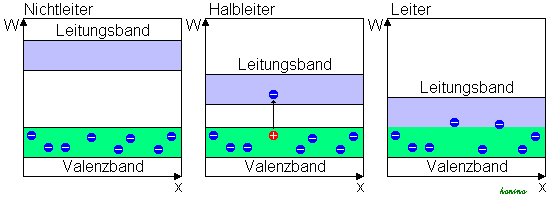
\includegraphics[width=0.8\textwidth]{images/Bandstruktur.png}
    \caption{Schematische Darstellung der unterschiedlichen Bandstrukturen. Links ist die Bandstruktur eines Isolators, 
    in der Mitte die eines Halbleiter und rechts eines Metalls abgebildet \cite{BS}.}
    \label{fig:Bandstrukturen}
\end{figure} \noindent
Es wird deutlich, dass bei einem Isolator, der auf der rechten Seite abgebildet ist, ein Abstand zwischen 
dem Leitungs- und dem Valenzband vorliegt. Diese wird als Bandlücke bezeichnet. Bei einem Isolator ist diese
Bandlücke zu groß, um sie allein mithilfe von thermischer Energie überwinden zu können. Das hat zur Folge, 
dass keine Elektronen in das Leitungsband gehoben werden und somit eine elektrische Leitfähigkeit erzeugen könnten. 
Bei einem Halbleiter, wie es auch Galium-Arsenit ist, liegt ebenfalls eine Bandlücke vor. Diese ist im Vergleich 
zu der eines Isolators kleiner. Somit können hier mithilfe von thermischer Energie Elektronen in das Leitungsband 
gehoben werden und das entsprechende Material wird leitend. Mithilfe von Dotierungen können die Bandlücken 
von Halbleitern verkleinert werden. Dazu werden Ladungsträger in das Material eingefügt. Dabei wird zwischen 
n- und p-Dotierung unterschieden. Bei einer n-Dotierung werden Elektronen-Donatoren, wohingegen bei einer p-Dotierung
Elektronen-Akzeptoren in das Material eingefügt. Diese sorgen dann für eine veränderte Bandstruktur, diese 
ist in Abbildung \ref{fig:BS_neu} dargestellt. \\
\begin{figure}[H]
    \centering
    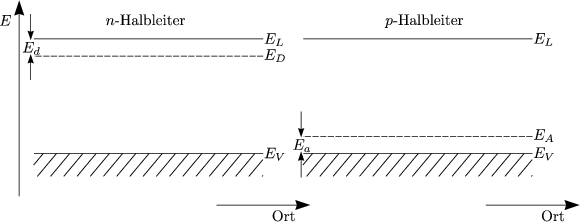
\includegraphics[width=0.8\textwidth]{images/BS_neu.png}
    \caption{Abbildung der durch eine Dotierung veränderten Bandstruktur eines Halbleiters. Links ist die n-Dotierung und rechts 
    die p-Dotierung dargestellt \cite{BS_neu}.}
    \label{}
\end{figure} \noindent
Bei einem Metall liegt kein Bandlücke vor. Außerdem ist das Leitungsband bereits zum Teil gefüllt. Somit reichen
bereits beliebig kleine Feldstärken aus, damit Elektronen in einen höheren Zustand übergehen können. Sie können 
als frei angenommen werden. 

\subsection{Faraday-Effekt}
Der Faraday-Effekt beschreibt die Drehung der Polarisationsrichtung einer einfallenden linear 
polarisierten Welle unter dem Einfluss eines magnetischen Feldes. Eine linear polarisierte Welle 
kann als Überlagerung zweier zirkular polarisierter Wellen angenommen werden. Tritt eine solche Welle in 
ein optisch anisotropes Medium so kommt es aufgrund der verschiedenen Phasenkomponenten der zirkularen
Komponenten zu einer Drehung der Polarisationsebene. Bei dem Eintritt in das Medium weist die Welle 
lediglich eine Komponente in eine Raumrichtung auf. Nach dem Durchlauf kommt es aufgrund der Drehung 
zusätzlich zu einem Beitrag in eine weitere Raumrichtung. Die Polarisationsrichtung ist somit um den 
Winkel $\theta$ gedreht. Aufgrund der unterschiedlichen Phasengeschwindigkeiten liegen ebenfalls 
unterschiedliche Brechungsindices vor. Aufgrund dessen wird in diesem Zusammenhand auch oftmals von einer 
Doppelbrechung gesprochen. Diese entsteht aufgrund der Die Doppelbrechung entsteht 
durch die Wechselwirkung der Bandelektronen mit den Rümpfen der Atome und 
den elektrische Dipolmomente der Atome auf den Gitterplätzen des Kristalls. \\
Mathematisch wird dieser Vorgang durch den Suszeptibilitätstensor beschrieben. Bei den zuvor beschriebenen 
anisotropen Medien handelt es sich dabei um einen Tensor mit Einträgen auf der Haupt- und den Nebendiagonalen. 
Die Einträge auf den Nebendiagonalen sind dabei die komplex konjugierten der Hauptdiagonaleneinträge. \\
\par 
Der Faraday-Effekt ist jedoch nicht außschließlich bei den zuvor erwähnten anisotropen Medien zu beobachten. 
Liegt ein Festkörper vor, der ausschließlich Einträge auf der Hauptdiagolen besitzt, findet ein 
Magnetfeld Anwendung. Durch Verwendung diese Magnetfeldes kommt es dazu, dass das Material doppelbrechend wird 
und ebenfalls komplex konjugierte Einträge erhält. Daraus folgt, dass der Drehwinkel $\theta$ 
proportional zur Flussdichte B, der Länge des Kristalls L und zur Anzahl der Ladungsträger pro Volumeneinheit N
ist. Somit ergibt sich 
\begin{equation}
    \theta = \frac{e_0^3 \lambda ^2 N L B}{8 \pi^2 \epsilon_0 c^3 (m^*)^2 n}
    \label{eqn:effmass}
\end{equation} \noindent
für den Drehwinkel. Dabei beschreibt L die Länge der Probe, B die magnetische Flussdichte und N die 
Ladungsträgerdichte. Außerdem beschreibt $\lambda$ die Wellenlänge und $m^*$ die effektive Masse der
Ladungsträger. Diese kommt zum Einsatz, da sie im Gegensatz zu der Elektronenmasse die Einflüsse des 
Gitterpotentials im Kristall bercksichtigt. Dazu betrachtet sie die Ladungsträger wie freie Elektronen bzw. 
Löcher im Vakuum, lediglich mit einer anderen Masse. Somit ist es mithilfe des Faraday-Effektes und Bestimmung
der Drehwinkel möglich die effektive Masse der Ladungsträger zu bestimmen.